%!TEX root = ../Thesis.tex
\section{Projektplanung}

\subsection{Vorgehensweise [Gentges]}

In der Projektplanung sollte die grundlegende Struktur für das weitere Vorgehen festgelegt werden. Zunächst sollte im Kapitel 4.2 der Funktionsumfang beschrieben, um ein einheitliches Verständnis darüber zu bekommen, welche Funktionen die Applikation später erfüllen muss und für welches Betriebssystem diese entwickelt wird. 

Im Projektablaufplan (Kapitel 4.3) werden die in der Planung obligatorischen Dokumente, wie z.B. ein Projektstrukturplan oder ein GANTT-Diagramm, sowie das Verfahrensmodell beschrieben.

Im Kapitel 4.4 wird das Planungsvorgehen der Software erläutert, neben der Planung des Mockups wird hierbei ebenfalls auf die Planung des Design Patterns eingegangen.

Anschließend werden die vorliegenden Datenstrukturen und Schnittstellen beschrieben. 

Danach wird die persistente Datenhaltung auf das Projekt angewendet und beschrieben. 

Zuletzt wird neben der Planung des Presenters, der View sowie der eigentlichen Menüsteuerung eine grobe Übersicht über die geplante Aufgabenverteilung im Team gegeben. 

\clearpage

\subsection{Funktionsumfangs [Falk]}

Im Rahmen dieses Projekts muss eine Android-App entwickelten werden, welche die Funktion eines kachelbasierten UPN-Taschenrechners zur Verfügung stellt. 

Dabei müssen drei verschiedene Kacheltypen implementiert werden: \textit{Operator}, \textit{Operand} und \textit{CalculatorFunction}. Ein Operator kann hier zum Beispiel die Wurzel oder Division sein und kann eine beliebige Stelligkeit aufweisen. Ein Beispiel für einen Operanden wären Dezimalzahlen oder Matrizen. Die CalculatorFunction-Kachel kann verschiedene Einstellungen bereitstellen. Dazu zählen u.a. Speicherung eines Layouts, Festlegung des Typs einer Kachel. Jede Kachel muss veränderbar sein und jede Rolle annehmen können. Eine Kachel darf nicht grundsätzlich gesperrt sein. 

Die Rechnungen sollen in einer bestimmten Reihenfolge geschehen. Zuerst wählt man die Kachel(n) aus, die den(die) benötigten Operanden beinhalten, dann die Kachel, in welche das Ergebnis geschrieben werden soll und schlussendlich sollte die Operation durchgeführt werden. Die ersten beiden Schritte können unter Umständen entfallen. 

Ein grober Überblick über die zu implementierenden Aktionen des Nutzers sind  nachfolgend dargestellt.

\begin{figure}[h]
	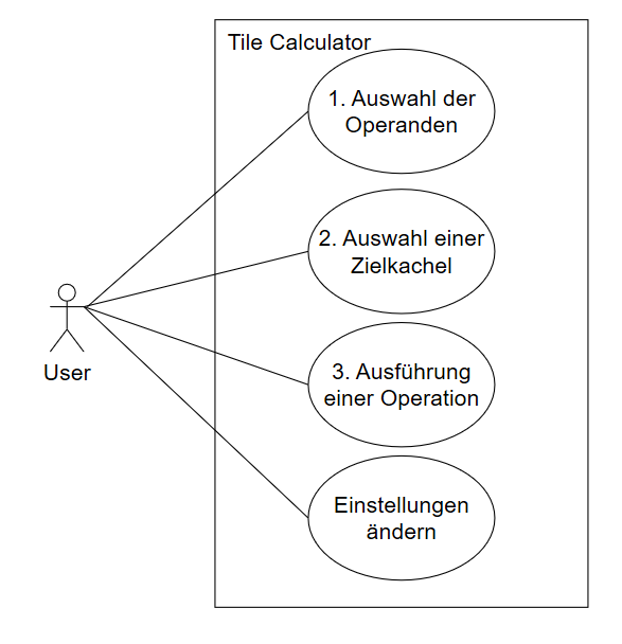
\includegraphics[width=0.75\columnwidth]{img/funktionsumfang-grundanforderungen-use-case-diagramm}
	\caption[Grundanforderungen Use-Case-Diagramm]{Grundanforderungen Use-Case-Diagramm\footnotemark}
\end{figure}
\footnotetext{eigene Darstellung}

Während der Bearbeitung des Projekts soll ein besonderes Augenmerk auf drei Aspekte gelegt werden. Der erste ist die komfortable Festlegung von Operanden-Kacheln. Dazu zählt auch das Ändern selbiger und derer Reigenfolge. Der zweite Punkt ist die Konfiguration der Ergebniskacheln. Der dritte Punkt sagt aus, dass die App so benutzerfreundlich wie möglich gestaltet werden soll. Dies soll zum Beispiel durch intuitive Bedienung, minimale Userinteraktion und übersichtliche Gestaltung erreicht werden. 

Die App soll für Android in Java entwickelt werden. Prinzipien des objektorientierten Software Entwurfs sollen hierbei eingehalten werden. Während der Durchführung des Projektes soll das Team nach dem erweiterten Wasserfallmodell arbeiten. Nach Möglichkeit sollen etablierte Entwurfsmuster eingesetzt werden. Es soll eine strikte und stark ausgeprägte Modularisierung durchgeführt werden. Hierbei soll die App das Samsung Galaxy Note 8.0 unterstützten. Die Unterstützung weiterer Geräte ist optional. Sowohl der Portrait Modus als auch der Landscape Modus sollen unterstützt werden. Ein Wechsel während der Nutzung der App soll möglich sein. Generell sollen Änderungen der Konfiguration des Androidsystems während der App-Ausführung unterstützt werden. Das Projekt soll in Android Studio importiert werden können. Der Import soll lokal, das heißt ohne eine bestehende Netzwerkverbindung möglich sein.

\begin{figure}[h]
	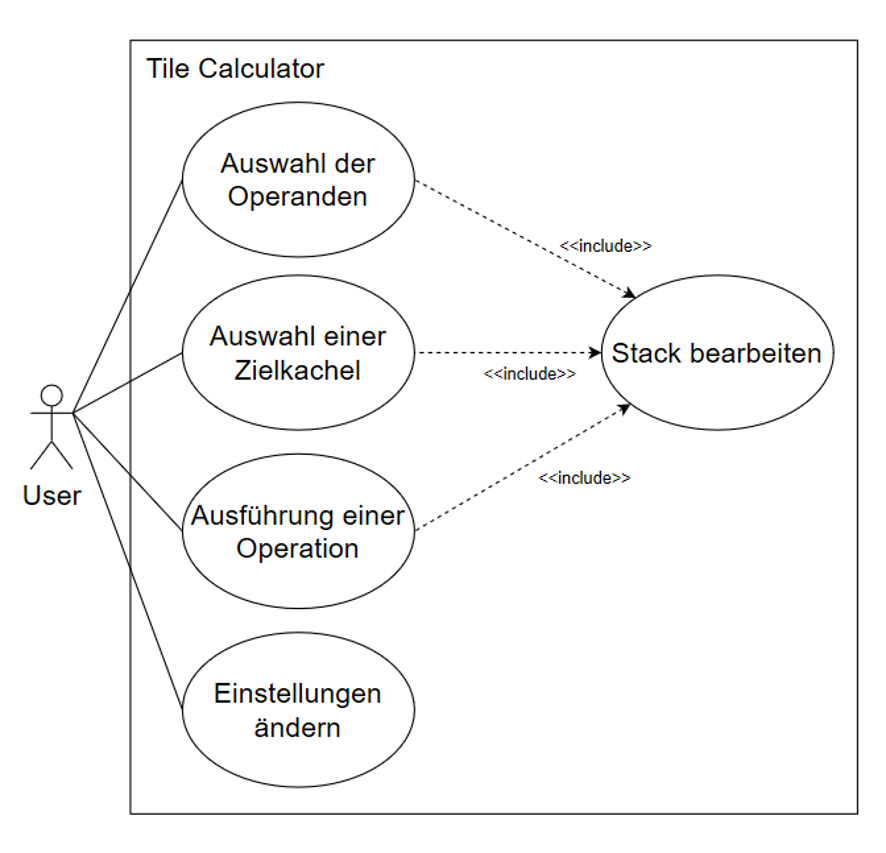
\includegraphics[width=0.9\columnwidth]{img/funktionsumfang-grobe-darstellung-der-funktionen}
	\caption[Grobe Darstellung der Funktionen]{Grobe Darstellung der Funktionen\footnotemark}
\end{figure}
\footnotetext{eigene Darstellung}

\subsection{Projektablaufplan [Gentges]}

Am Anfang musste ein geeignetes Vorgehensmodell ausgewählt werden. Dabei wählte ich als Projektleiter das erweiterte Wasserfallmodell. Die eindeutigen Argumente für dieses Modell waren zum einen die klare Struktur und der geringe Managementaufwand. Weiterhin war die gute Übersichtlichkeit und eine einfache Verständlichkeit ein klarer Vorteil gegenüber anderen Modellen, wie z.B. SCRUM. Außerdem ist das erweiterte Wasserfallmodell sehr gut geeignet für kleinere Projekte mit genau definiertem Umfang.

Für das vorliegende Projekt wurde das erweiterte Wasserfallmodell mit 8 Phasen ausgewählt. 

\begin{figure}[h]
	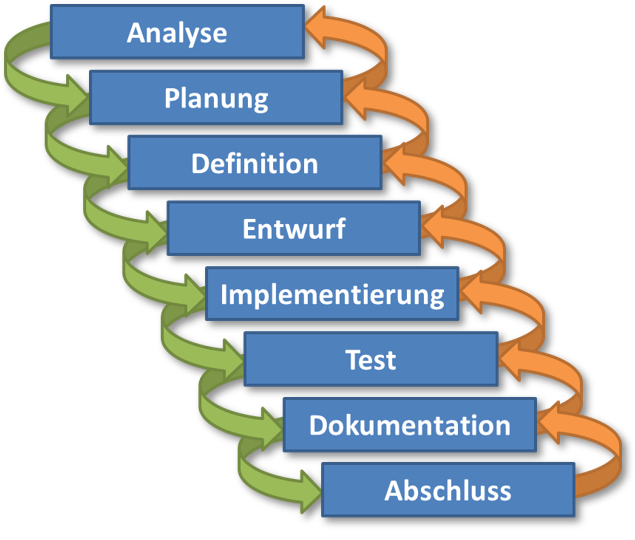
\includegraphics[width=0.8\columnwidth]{img/projektablaufplan-erweitertes-wasserfallmodell}
	\caption[Erweitertes Wasserfallmodell]{Erweitertes Wasserfallmodell\footnotemark}
\end{figure}
\footnotetext{eigene Darstellung}

''Es ist ein lineares Vorgehensmodell in der Softwareentwicklung, bei dem der Softwareentwicklungsprozess in einzelnen, festen Phasen organisiert wird. Dabei gelten die Phasenergebnisse immer als bindende Vorgaben für die nächste Phase.''\footnote{\cite[][]{itemis2015}}

Bei dem erweiterten Wasserfallmodell sind, begleitend zu der kontinuierlichen Kontrolle des Projektfortschritts, Rücksprünge in die vorherige Bearbeitungsphase möglich, sollte z.B. ein Fehler in einer nachfolgenden Phase identifiziert werden. Das erweitere Wasserfallmodell bietet eine gute Sicht über den gesamten Projektablauf, da alle Aktivitäten einer Phase vorerst vollständig abgeschlossen werden müssen, bevor man in die darauffolgende Phase übergeht.

Auf diesem Vorgehensmodell basierte die Projektstrukturplanung, die Meilensteinplanung sowie die Zeitplanung, welche in einem GANTT-Diagramm visualisiert wurde.

Der Projektstrukturplan gliedert sich in mehrere Teilprojekte mit jeweils dazugehörigen Arbeitspaketen.

''Der Projektstrukturplan ist die vollständige Darstellung aller Elemente eines Projektes und ihrer Beziehungen. Dabei werden die Elemente hierarchisch gegliedert, so dass eine Baumstruktur entsteht.''\footnote{\cite[][]{andreawindolph}}

Den einzelnen Arbeitspaketen und Teilaufgaben sind weitere, kleinere Arbeitspakete und Teilaufgaben zugewiesen. 

\clearpage

\interfootnotelinepenalty=10000

\enlargethispage{3\baselineskip}

\begin{figure}[!h]
	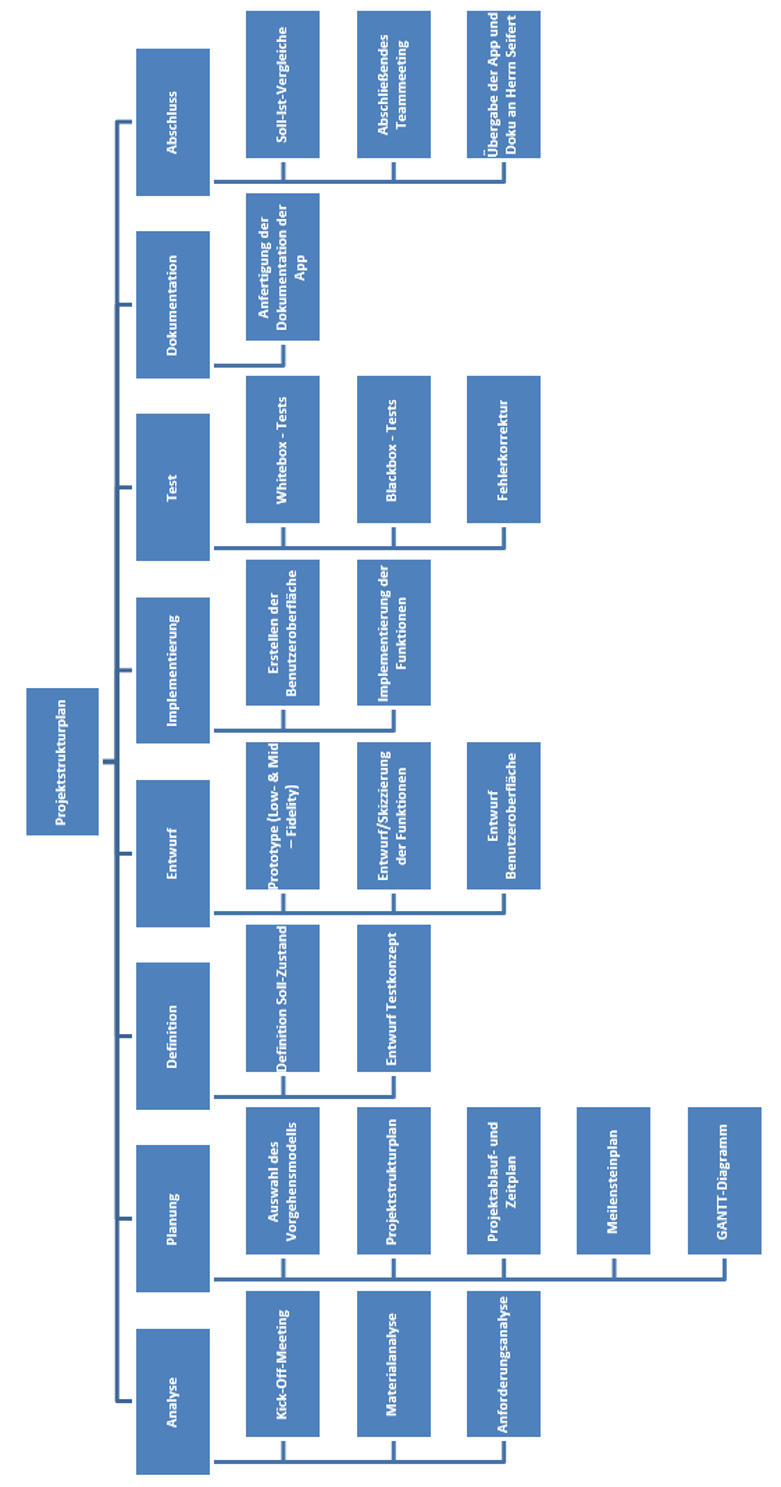
\includegraphics[width=\textwidth,height=50em,keepaspectratio]{img/projektablaufplan-psp}
	\caption[Projektstrukturplan]{Projektstrukturplan\footnotemark}
\end{figure}
\footnotetext{eigene Darstellung}

\clearpage

\interfootnotelinepenalty=100

\begin{tabularx}{\textwidth}{|p{2em}|X|p{5em}|}
\hline
\textbf{ID} & \textbf{Meilenstein} & \textbf{Datum} 
\\ \hline \hline
1 &Kick-Off Meeting abgehalten &	03.09.2019
\\ \hline
2&	Vorgehensmodell ausgewählt&	04.09.2019
\\ \hline
3&	Zeitplanung (GANTT) und Kommunikation&	04.09.2019
\\ \hline
4&	Aufgabenverteilung	&05.09.2019
\\ \hline
5&	Mockups fertiggestellt&	04.01.2020
\\ \hline
6&	Android Studio Implementierung&	25.01.2020
\\ \hline
7&	App getestet&	28.01.2020
\\ \hline
8&	Finale App Version&	04.02.2020
\\ \hline
9&	Dokumentation fertig&	05.02.2020
\\ \hline
10&	Abgabe der Ausarbeitung bei Herrn Seifert&	06.02.2020
\\ \hline
11&	Präsentation&	08.02.2020
\\ \hline
\end{tabularx}

''Meilensteine gliedern und strukturieren Projekte. Ein Meilensteinplan ist ein häufig genutztes Werkzeug im Projektmanagement und zeigt die Meilensteine eines oder mehrerer Projekte in chronologischer Reihung an.''\footnote{\cite[][]{t2informatik}}

Der Meilensteinplan wurde dabei unmittelbar nach dem Kick-Off Meeting an das Team kommuniziert. Dabei konnten die Daten der Meilensteine eingehalten werden. Zusammenfassend wird dies in einem Soll-Ist-Vergleich von meinem Kollegen Hendrik Falk näher beleuchtet.

GANTT Diagramme sind im Projektmanagement ein gängiges Tool, um Aktivitäten in Relation mit der Zeit zu setzen. Das Diagramm enthält eine Auflistung von Aktivitäten mit zugewiesenen Zeitleisten.\footnote{\cite[vgl.][]{ganttGentgesxy2001a}}

\clearpage

\interfootnotelinepenalty=10000

\enlargethispage{3\baselineskip}

\begin{figure}[!h]
	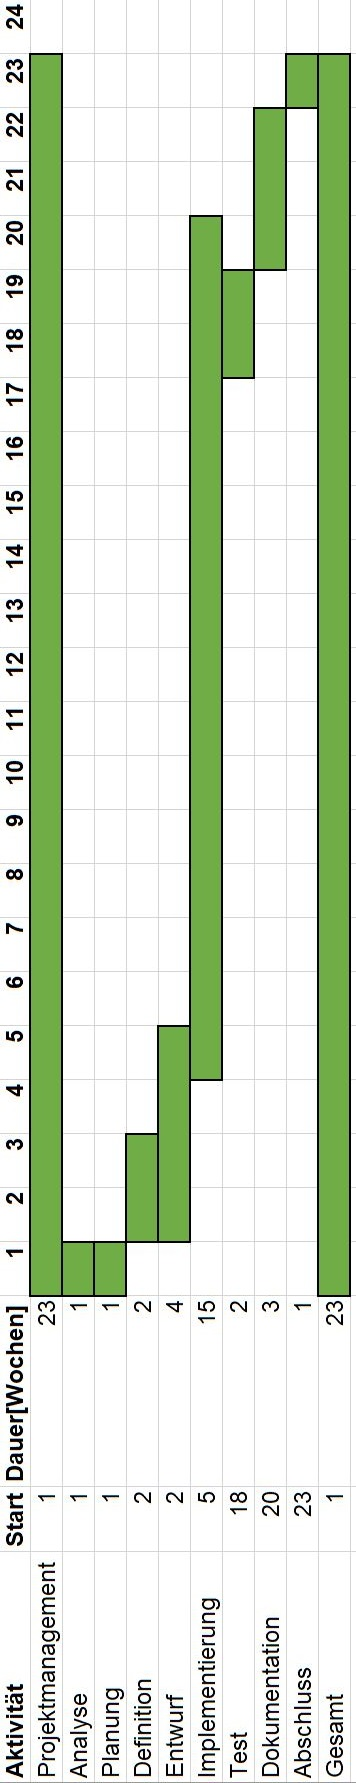
\includegraphics[width=\textwidth,height=50em,keepaspectratio]{img/projektablaufplan-gantt}
	\caption[GANTT-Diagramm]{GANTT-Diagramm\footnotemark}
\end{figure}
\footnotetext{eigene Darstellung}

\clearpage

\interfootnotelinepenalty=100

\subsection{Planung der Software}

\subsubsection{Planung des Mockups [Pham]}

Um ein erstes Konzept für eine mögliche Umsetzung des Projektes zu erstellen, wurde zunächst ein Mockup in Form eines Paper-Prototyps erstellt. Bei der Erstellung des Mockups sollten die grundlegenden Regeln des Usability Engineerings eingehalten werden. Unter Usability Engineering ''versteht man den Prozess, der parallel zur klassischen Planungs- und Entwicklungsarbeit die spätere Gebrauchstauglichkeit eines Systems sicherstellt.''\footnote{\cite[][S.~204]{handbuchusability2007}} Das heißt, um für eine möglichst hohe Usability des Endproduktes zu sorgen, wurden bereits während der Konzeptionierung des Mockups Usability Aspekte mit in Betrachtung gezogen. 

Um sicherstellen zu können, dass das Konzept für die Umsetzung des Projektes sich mit den Vorstellungen des späteren Benutzers und Auftraggeber (Prof. Dr. Thomas Seifert) deckt, wurde das gegebene Material analysiert sowie ein Gespräch mit dem Benutzer geführt, um die generellen Anforderungen ableiten zu können. 

Die spezifischen Anforderungen, die sich während des Interviews ergaben, wurden dabei dokumentiert und mithilfe der gesammelten Anforderungen konnte der erste Low-Fidelity Paper Prototyp erstellt werden.

\interfootnotelinepenalty=10000

\begin{figure}[!h]
	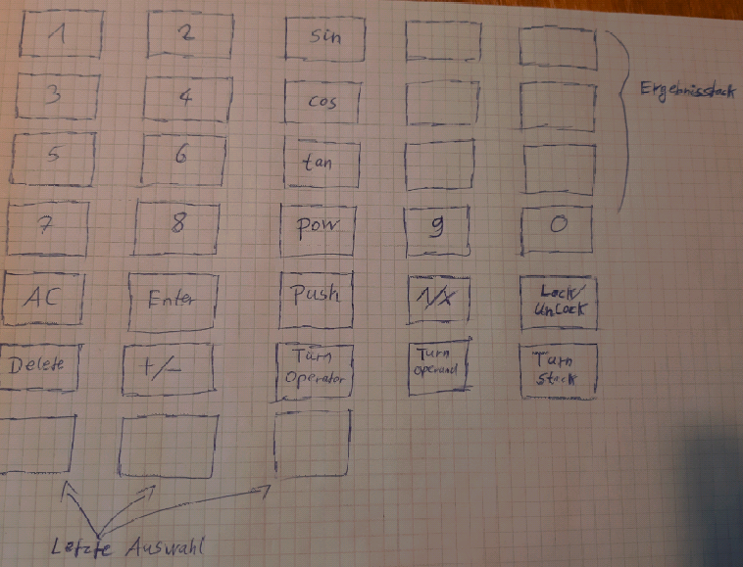
\includegraphics[width=1\columnwidth]{img/planung-mockup-erster-mockup}
	\caption[Erster Paper Prototype]{Erster Paper Prototype\footnotemark}
\end{figure}
\footnotetext{eigene Darstellung}

\interfootnotelinepenalty=100

Ein Low-Fidelity Prototyp dient hierbei lediglich als ein erstes Proof of concept, in dem das grundlegende Konzept und das erste Design festgehalten werden sollen. Eine Funktionalität des Konzeptes ist hierbei nicht notwendig.\footnote{\cite[vgl.][S.~204]{jhammondtgrossjwesson2002}}

Auf die genaueren Details des Low-Fidelity Paper Prototyp wird in Kapitel 7.1.5.3 XXX„Erstellung des Low-Fidelity ‚Paper Prototyps‘ “ eingegangen. Ziel des Low-Fidelity Paper Prototyps war es, mit möglichst geringem Aufwand so nah wie möglich an die Vorstellungen des Benutzers zu kommen und den Prototypen iterativ zu verbessern. Aus diesem Grund wurde das erste entwickelte Mockup dem Benutzer erneut präsentiert, um Feedback einzuholen und das Konzept iterativ verbessern zu können. Die dabei identifizierten Diskrepanzen zwischen dem Konzept und den Vorstellungen des Benutzers wurden festgehalten und mithilfe des gesammelten Feedbacks konnte ein zweiter Paper Prototyp erstellt werden. Nachdem die Zwischenergebnisse mit dem Benutzer verifiziert wurde, wurde ein Mid-Fidelity Prototype in MS PowerPoint angefertigt.

Der Mid-Fidelity-Prototyp ist hierbei interaktiv, relativ detailliert und simuliert das erwünschte Verhalten des finalen Produktes. Es soll im Mid-Fidelity-Prototyp bereits auf Aspekte wie Funktionalität, finales Design oder Navigation eingegangen werden.\footnote{\cite[vgl.][S.~204]{jhammondtgrossjwesson2002}}

\interfootnotelinepenalty=10000

\begin{figure}[!h]
	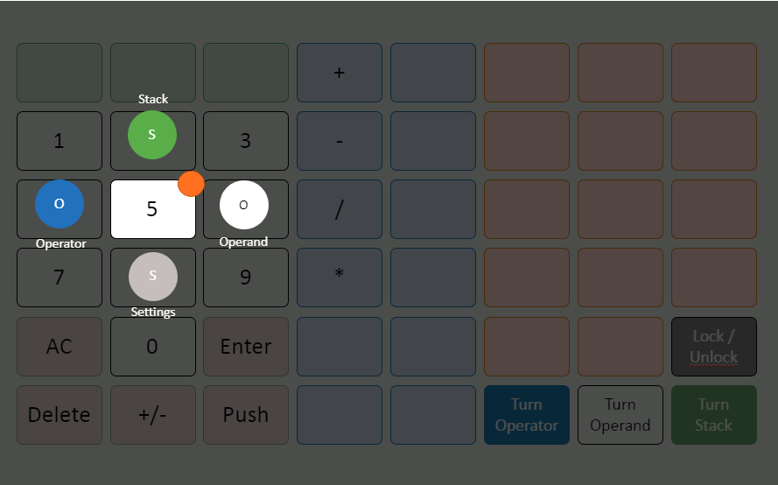
\includegraphics[width=1\columnwidth]{img/planung-mid-fidelity}
	\caption[Mid-Fidelity Prototyp]{Mid-Fidelity Prototyp\footnotemark}
\end{figure}
\footnotetext{eigene Darstellung}

\interfootnotelinepenalty=100

Im Beispiel unseres Mid-Fidelity Prototyps wurde genauer auf die Umsetzung des Kachelkonzept des Taschenrechners eingegangen ebenso wie die Anforderung für die ''Minimierung der Anzahl der für die Ausführung einer Rechnung erforderlichen Interaktionen'' mithilfe einer hohen Usability umgesetzt werden sollte. Auf diese Aspekte des Mid-Fidelity Paper Prototyp wird näher in Kapitel XXX 7.1.3.1	„Erstellung der Funktionalitäten des Mid-Fidelity Prototyps“ eingegangen. 

Weiterhin wurde ein Standardlayout für den Taschenrechner entworfen und designt, welches beim Aufruf des Taschenrechners angezeigt werden sollte. Detaillierter wird dieses Design in Kapitel XXX 7.1.7.1	''Erstellung des Design Konzeptes des Mid-Fidelity Prototyps'' beschrieben. 

Insgesamt ließ sich bei dem Mid-Fidelity-Prototyp das geplante Layout bereits sehr detailliert visualisieren, so dass eine Umsetzung und das finale Design in Android Studio auf Basis des Prototyps bereits möglich gewesen wären. Auch konnten durch die Interaktionsfähigkeit des Prototyps die verschiedenen Use-Cases interaktiv durchgespielt und getestet werden. Nach Fertigstellung des Mid-Fidelity-Prototyps in PowerPoint durch das GUI-Team, wurde das Design und das allgemeine Benutzeroberflächenkonzept des Prototyps dem gesamten Projekt-Team vorgestellt und anschließend vom allen Teammitgliedern in einem der Zwischen-Meetings abgesegnet. 

Damit war ein detailliertes Konzept der geplanten Applikation erstellt und der Mid-Fidelity-Prototyp konnte als Basis für die weitere Entwicklung der Applikation verwendet werden. 

\clearpage

\subsubsection{Planung der Design Patterns [Falk]}

Die Teammitglieder suchten einen sinnvollen Ansatz, wie es möglich ist, die Software in verschiedenen Komponenten zu unterteilen und damit sowohl Kollaboration, als auch einfache Verständlichkeit gewährleistet werden können. Design Pattern dienen grundsätzlich der Lösung wiederkehrender Entwurfsprobleme. Außerdem geben sie einem die Möglichkeit, Gebrauch von vielen Best Practices zu machen, z.B. derer der \textit{Gang of Four}. 

In diesem Projektabschnitt wurden User Interface Design Pattern betrachtet. Die Anwendung dieser Pattern dient der Trennung von UI Designern, welche sich dadurch auf die Nutzererfahrung und das Aussehen kümmern können, und Back-End-Entwicklern, damit diese sich dann auf die technische Umsetzung konzentrieren können. 

Die Teammitglieder betrachteten hierzu verschiedenen MVx Pattern. Dabei steht das ''M'' für Model, also die tatsächliche Businesslogik der Applikation (tatsächliche Rechenoperationen) und das ''V'' für View, also die Ansicht, die der Endnutzer sieht. Das ''x'' steht für ein kommunikatives Bindeglied, was je nach Implementierung variiert. Diese haben ihren Ursprung im Jahre 1979, in welchem Trygve Reenskaug das Model View Controller (MVC)-Pattern entwarf.\footnote{\cite[vgl.][]{c2MVC}} Aus diesem Pattern entwickelte sich auch das Model View Presenter (MVP)-Pattern. Dieses wurden bereits in den 1990er Jahren eingesetzt, die ausschlaggebende Definition stammt jedoch von Martin Fowler aus dem Jahre 2004.\footnote{\cite[vgl.][]{FowlerMVP}} Ein Jahr später, 2005, veröffentlichte John Gossmann dann das Model View Viewmodel (MVVM)-Pattern.\footnote{\cite[vgl.][]{HeiseMVVM}}

Jede Implementierung weißt eine unterschiedliche Kommunikation zwischen den Komponenten auf. Der Ursprung dessen liegt darin, dass die Komponenten unterschiedliche Wissensstatus aufweisen, also ob die Instanzen der anderen Komponenten übergeben wurden oder nicht. 

Die einzelnen Komponenten kommunizieren entweder über direkte Zugriffe auf Attribute und Methoden miteinander oder aber indirekt. Indirekte Kommunikation findet z.B. über die Rückgabewerte Methoden statischer Klassen oder aber über Events durch das Observer Pattern statt. Nach dem Observer Pattern würde Beispielsweise ein Presenter ein Beobachter für das Model, welches das Subjekt wäre. Dabei informiert das Subjekt den Beobachter über seine Veränderungen. 
Zuerst betrachteten die Teammitglieder das modernste dieser Pattern, das MVVM-Pattern. Zur Erklärung der Pattern werden Diagramme verwendet, welche eine Mögliche Umsetzung der Pattern darstellen.

\interfootnotelinepenalty=10000

\begin{figure}[!h]
	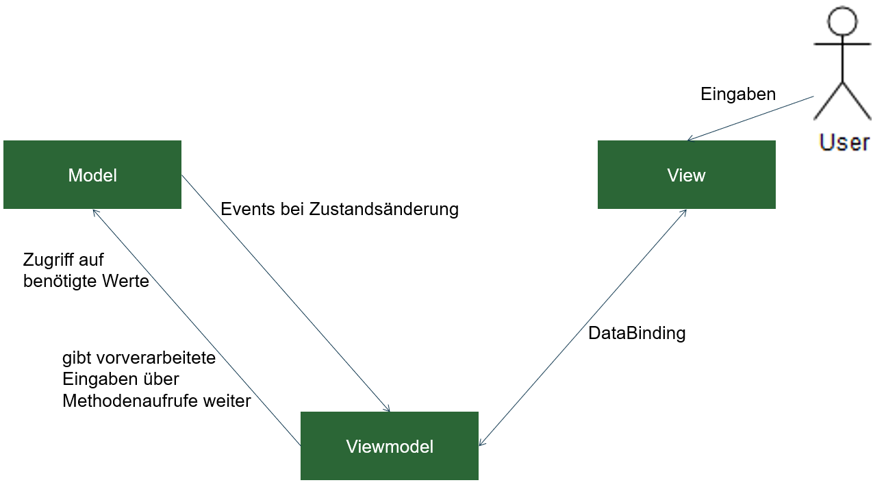
\includegraphics[width=1\columnwidth]{img/design-pattern-mvvm}
	\caption[Mögliche Umsetzung von MVVM ]{Mögliche Umsetzung von MVVM\footnotemark}
\end{figure}
\footnotetext{eigene Darstellung}

\interfootnotelinepenalty=100

Der User interagiert in jedem Design Pattern mit der View und gibt dort seine Eingaben ein. An diesem Diagramm sieht man, dass bei MVVM die Kommunikation von Model zu Viewmodel über das Observer Pattern funktioniert und das Viewmodel direkt Methode aus dem Model aufruft. Viewmodel und View kommunizieren über DataBinding. Dabei werden Attribute des Viewmodels direkt mit Feldern der View verbunden. Dies führt dazu, dass man in der View lediglich die Anmeldung dieser Felder beim Viewmodel implementiert werden muss. Dieses Pattern kann teilweise bei der Implementierung des Viewmodels sehr kompliziert sein, bietet aber dafür die loseste Kopplung zu der View. Da eine so strenge Trennung für dieses Projekt allerdings nicht benötigt wurde, entschieden sich die Teammitglieder gegen dieses Pattern und betrachteten die nächsten Pattern MVP und MVC. 

\interfootnotelinepenalty=10000

\begin{figure}[!h]
	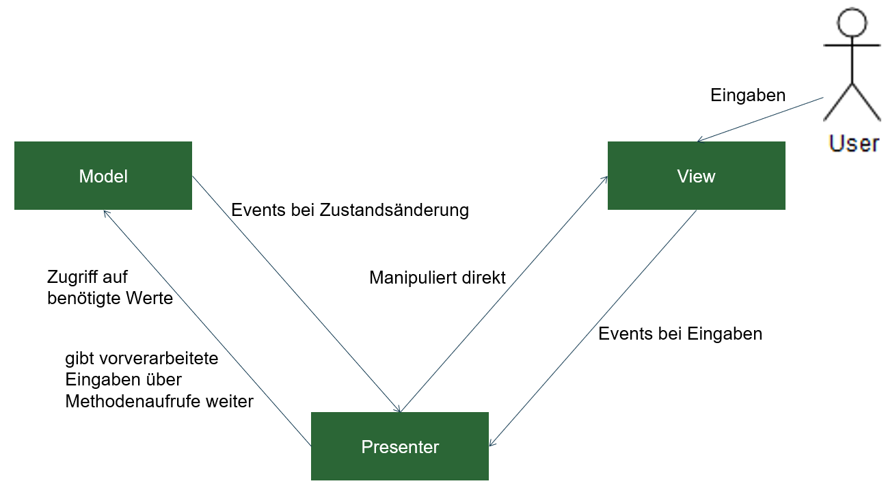
\includegraphics[width=1\columnwidth]{img/design-pattern-moeglich-mvp}
	\caption[Mögliche Umsetzung von MVP]{Mögliche Umsetzung von MVP\footnotemark}
\end{figure}
\footnotetext{eigene Darstellung}

\begin{figure}[!h]
	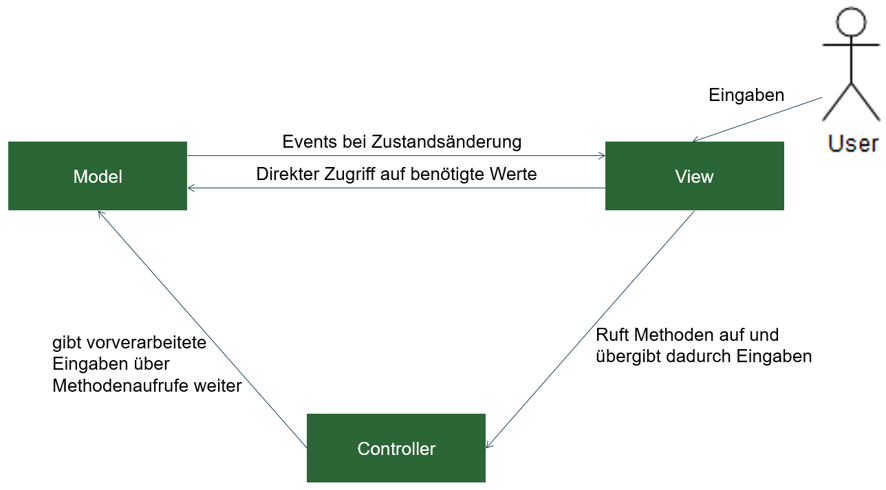
\includegraphics[width=1\columnwidth]{img/design-pattern-moeglich-mvc}
	\caption[Mögliche Umsetzung von MVC]{Mögliche Umsetzung von MVC\footnotemark}
\end{figure}
\footnotetext{eigene Darstellung}

\interfootnotelinepenalty=100

An den Darstellungen kann man sehen, dass sich die MVP und MVC Pattern sehr stark ähneln. Es unterscheidet sich nur die Kommunikation zwischen Model und View. Während beim MVC Pattern Model und View direkt miteinander kommunizieren, findet dies beim MVP Pattern über den Presenter statt. Aufgrund der hier kleinen Projektgröße war Simplizität ein sehr wichtiges Kriterium bei der Auswahl des UI Design Patterns. Da Android Usereingaben eventgetrieben verarbeitet, hielten die Teammitglieder eine MVP Implementierung für die geeignetste Lösung dieses Problems.

\clearpage

\paragraph{Singleton Pattern [Schwenke] XXX}

XXX

\clearpage

\paragraph{Factory Loader Pattern [Bockhorn] XXX}

XXX

\clearpage

\subsubsection{Planung der Datenstrukturen und Schnittstellen}

\interfootnotelinepenalty=10000

\enlargethispage{3\baselineskip}

\begin{figure}[!h]
	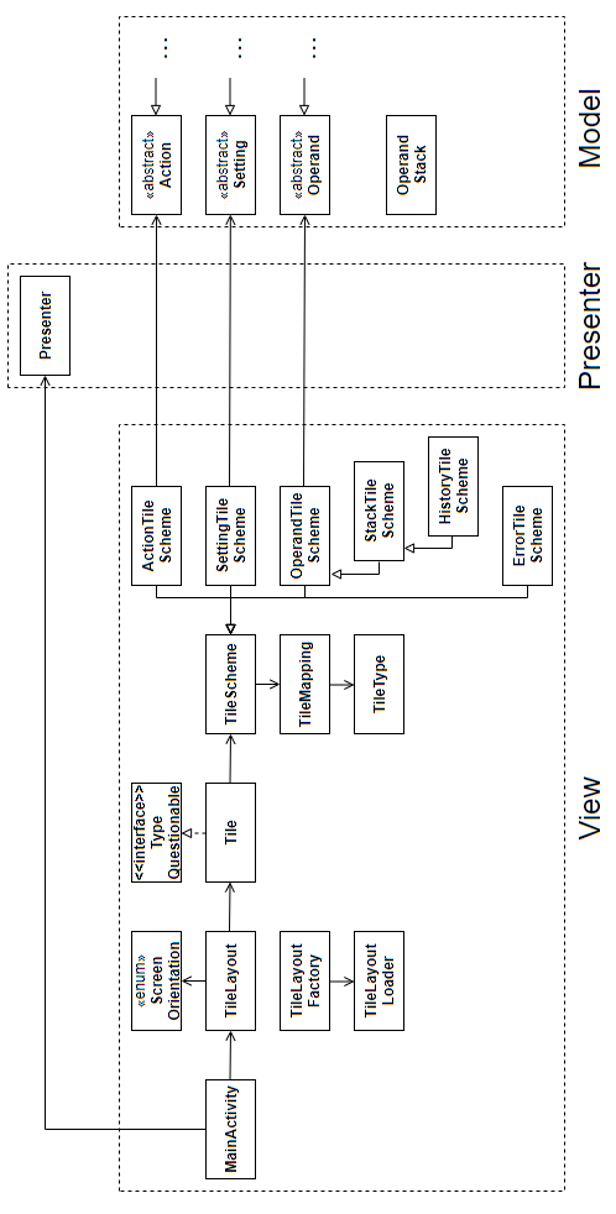
\includegraphics[width=\textwidth,height=50em,keepaspectratio]{img/schnittstellen-klassendiagramm}
	\caption[Klassendiagramm]{Klassendiagramm XXX\footnotemark}
\end{figure}
\footnotetext{eigene Darstellung}

\interfootnotelinepenalty=100

\clearpage

\para{Nutzung von Stack für Notation [Schwenke]}
Der Taschenrechner soll als Eingabelogik für die Anwendung von Operationen die umgekehrte polnische Notation verwenden. Hierbei werden immer zunächst die Operanden und im Anschluss daran die darauf auszuführenden Operatoren angegeben. Dieser Ansatz ermöglicht eine stapelbasierte Abarbeitung. 

Stacks werden, wie von den meisten Programmiersprachen, auch in Java in der Standardbibliothek unterstützt. Mit dabei sind Methoden wie \code{push} (für das Ablegen eines Objekts auf dem Stapel), \code{pop} (für das Entfernen und die Wiedergabe eines Objekts auf dem Stapel), \code{peek} (für die Wiedergabe ohne Entfernen eines Objekts auf dem Stapel) und \code{empty} (für das Leeren des Stapels). 

Jedoch müssen hierbei die besonderen Anforderungen des Taschenrechners beachtet werden. Operanden können von gänzlich unterschiedlichem Typus sein, zum Beispiel eine einfache Dezimalzahl oder auch ein Tupel, und viele Operationen benötigen mehr als die ersten (maximal zwei) Operanden auf dem Stack. Möchte man Elemente vom Stapel entfernen, kann man \code{pop} mehrmals aufrufen. Aufwändiger hingegen wird es bei \code{peek}. Möchte man mehrere Elemente vom Stapel einsehen ohne diese zu entfernen, muss man bei der Arbeit mit dem vorhandenen Stack einen weiteren bereithalten, nur um zwischengespeicherte Elemente lagern zu können. Anders ist es nicht möglich \code{peek} auf mehrere Elemente gleichzeitig anzuwenden. Gerade das ist aber bei der App notwendig. Weitere Methoden, die bei der umgekehrten polnischen Notation oft benötigt werden, aber nicht implementiert sind, sind \code{reverse} (für die Vertauschung der ersten zwei Elemente auf dem Stack, was wichtig für nicht-kommutative Operationen ist), \code{rollUp} (das unterste Elemente wird an den ersten Platz geschoben, das erste Element an den zweiten Platz usw.) und \code{rollDown} (das unterste Elemente wird an den ersten Platz geschoben, das erste Element an den zweiten Platz usw.).

Aufgrund dessen soll für dieses Projekt ein eigener Stapel implementiert werden. Dieser soll die zuvor genannten Funktionen mit unterschiedlichen Parametertypen unterstützen. Dabei ist darauf zu achten, dass die Programmierung generisch erfolgt und das Stack nicht nur alle Typen von Operanden unterstützt, sondern auch für gänzlich andere Klassenbäume in der App verwendet werden kann.

\para{Ansatz der Kalkulationsorchestrierung [Schwenke]}
Die App soll den Umgang mit unterschiedlichen Operanden-Typen beherrschen. Die Addition zweier Matrizen funktioniert anders als die Addition von zwei einfachen Dezimalzahlen. Java verfügt nativ weder über die entsprechenden Operanden noch über die Methoden für die Kalkulation. Auch die ausgewählte Bibliothek ist nicht ohne weiteres in der Lage Operationen auf alle Kombinationen von Operanden im folgenden Format einheitlich anzuwenden:

\begin{figure}[bht]
	\begin{lstlisting}[caption=Konzept für Nutzung generischer Schnittstelle, label=list:konzept-fuer-nutzung-generischer-schnittstelle]
	Operation.mit(matrixOperand, dezimalOperand, dezimalOperand)
	\end{lstlisting}    
\end{figure}

Einheitlichkeit ist notwendig, damit im Frontend der Applikation keine Logik vorhanden sein muss, die entscheidet wie genau (auf Basis der Operanden-Typen) eine Operation umgesetzt wird. Deswegen muss eine einfache Schnittstelle entwickelt werden, die für den Nutzer nur zwei Drehschrauben bereitstellt. Dies ist zunächst die Auswahl der gewünschten Operation. Das kann z.B. das Symbol \code{+} als übliches Zeichen für Addition sein. Anschließend wird eine Reihe von Operanden übergeben. Dieser Aufruf sollte schließlich das Ergebnis in Form eines Operanden zurückgeben. Im Fall der Addition einer Matrix mit einer rationalen Zahl wäre dies wiederrum eine Matrix. Die korrekte Kalkulation soll also dynamisch bestimmt werden. Wichtig zu klären ist hier auch das Verhalten im Falle eines Fehlschlags. Nicht alle Kombinationen von Operanden können unterstützt werden. Die Verwendung von \textit{Optionals} (ein \code{Optional} ist ein Objekt, das man sich als Datenbehälter vorstellen kann, der entweder einen Wert enthält oder leer – aber nicht \code{null} sein kann) bietet sich hier zwar an, wird jedoch von Java in der verwendeten Android API-Version nicht unterstützt. Deswegen ist hier geplant sogenannte \textit{checked Exceptions} zu verwenden. Diese müssen bei der Verwendung explizit aufgefangen und weiterverarbeitet werden. Die Abbildung einer Operanden-Kombination auf die entsprechende konkrete Kalkulationsmethode muss dementsprechend zur Laufzeit des Programms erfolgen. Ein solches Mapping ist in Java nur mithilfe des Reflection-Pakets möglich. Reflektion ermöglicht den Einblick in ein Objekt (neben der Nutzung des Punkt-Operators) in eine Klasse. Zum Beispiel kann man eine Methode anhand einer Kombination von Parametertypen finden und aufrufen. Es ist geplant diesen Ansatz für die Orchestrierung der Kalkulationen in der App zu verwenden. Auch ist es nicht notwendig nur eine vordefinierte Anzahl an Argumente anzunehmen. So kann es sinnvoll sein, dass eine Methode zur Erstellung eines Tupels eine beliebige Anzahl an Operanden annimmt. Auch das lässt sich mit Reflektion umsetzen.

Der große Vorteil dabei ist, dass nirgendwo explizit in einer Abfrage entschieden werden muss, welche Kombination von Operanden an welche Methode weitergeleitet werden soll. Die Zuordnung erfolgt rein über die Deklaration der Parametertypen in der Methode selbst. Das macht das Ändern und Erweitern der Rechenfunktionalitäten einfach. Es muss lediglich die entsprechende Klasse herausgesucht und eine Methode im korrekten Format hinzugefügt werden. 

\paragraph{Persistente Datenhaltung\protect\footnote{\cite[vgl.][]{ogbo2016}} [Meinerzhagen]}

Im Rahmen der persistenten Datenspeicherung wurde zuerst betrachtet, was dauerhaft gespeichert werden muss und welche Elemente beim Start der Anwendung neu generiert werden können. Anschließend wurden die verfügbaren Speichermethoden betrachtet und im Anwendungskontext evaluiert. Die passendste Methode wurde letztlich ausgewählt.

Entsprechend den erarbeiteten Anforderungen wurden in diesem Bereich das Speichern und Laden des aktuellen Zustandes der Kacheln und deren Layout in den Vordergrund gesetzt. Das Layout soll einem Gitternetz entsprechend aufgebaut sein.

Zum Abspeichern dieser Daten wurden die verschiedenen Optionen betrachtet. Android bietet vier Varianten zur persistenten Datenspeicherung nativ an. Diese sind Shared Preferences, interne Speicher, externe Speicher und eine Datenbank. Mit Shared Preferences können einfache Key-Value-Paare gespeichert werden. Für diese wird automatisch eine Datei erstellt, welche Android verwaltet. Der interne Speicher bietet ein, vom restlichen Android System abgekapseltes, Dateisystem. Nur die App selbst ist erlaubt dort Daten zu speichern und lesen. Dagegen beschreibt der externe Speicher das bestehende Dateisystem von Android, auf welches der Nutzer und andere Apps freien Zugriff haben. Letztlich kann eine Datenbank zum Speichern verwendet werden. Android bietet dazu eine SQLite Datenbank an.

Auf Grund der tabellenähnlichen Struktur der zu speichernden Daten wurde zum Speichern ein Tabellenformat angedacht. Dabei fiel die Wahl auf das gängige CSV Format. Mit der Wahl dieses waren die Shared Preferences und die Datenbank nicht mehr nutzbar. Somit lag die Wahl zwischen dem internen und externen Speicher. Da ein Zugriff auf die gespeicherten Daten von außerhalb nicht notwendig ist, fiel die Wahl auf die Nutzung des internen Speichers. 

\clearpage

\subsubsection{Planung des Presenters [Tom]}

XXX

Der Presenter agiert als Bindeglied zwischen der View und dem Model, sodass alle Bereiche ihre Funktionalitäten im vollen Maß erfüllen können und eine Separierung der Anwenderschnittstelle und der Geschäftslogik gewährleistet werden kann. Der Presenter koordiniert die Kommunikation zwischen View und Model, also steuert Rechnungen im Backend und sorgt für die korrekte Darstellung der Ergebnisse in den einzelnen Kacheln der View.

Mit der View kommuniziert er über eine Container Klasse (XXX), welche die einzelnen Kacheln koordiniert. Aufrufe der View in Richtung des Presenters werden durch Events realisiert. Dabei wird die in Android native Listener Funktionalität verwendet, wobei der Presenter als \code{OnClickListener} dient. Er ist sich über die Instanz der Container Klasse bewusst und interagiert direkt mit dessen Attributen und Methoden.

Das Model besteht aus verschiedenen Klassen, welche die Kacheltypen aus den Vorgaben widerspiegeln. Da diese dezentral vorliegen und es gemäß der geplanten MVP-Implementierung hier zu einer sehr komplexen Struktur von Events kommen würde, wurde sich dazu entschieden, die Kommunikation von Model zu Presenter über Rückgabewerte einzelner Methoden zu gestalten. Die entgegengerichtete Kommunikation verläuft nach Entwurf, also über direkte Aufrufe von Methoden und Attributen. Die aktuellen Operanden im Stack und die zuvor eingetragenen Operanden in der Historie werden jeweils als Listen im Presenter geführt.

Um mit dem Presenter jegliche Eingabe verarbeiten zu können, wird diesem die Kachelidentität im Event übergeben. Diese wird ihm übergeben und er führt je nach Typ verschiedene Operationen durch.

\begin{itemize}
\item Bei Identifikation einer Kachel vom Typ Operand, wird dieser entweder an die aktuelle Eingabe zur Anlage von neuen Operanden angehängt, z.B. 2 und 3 zu 23, oder in den Stack und in die Historie geschoben. 
\item Bei einer Operation wird diese mit so vielen Operanden wie möglich ausgeführt und das Ergebnis in Stack und Historie geschoben.
\item Die Verarbeitung von Einstellung ist sehr individuell und nur gegebenenfalls werden Inhalte in Stack und Historie geschoben. Ein Beispiel für eine Einstellung ist die Taste \code{AC} (All Clear) im Taschenrechner. Diese entfernt jegliche Eingaben aus dem aktuellen Stack.
\item Identifiziert der Presenter eine Kachel vom Typ Stack oder Historie, so wird diese wie ein Operand behandelt.
\end{itemize}

\interfootnotelinepenalty=10000

\begin{figure}[!h]
	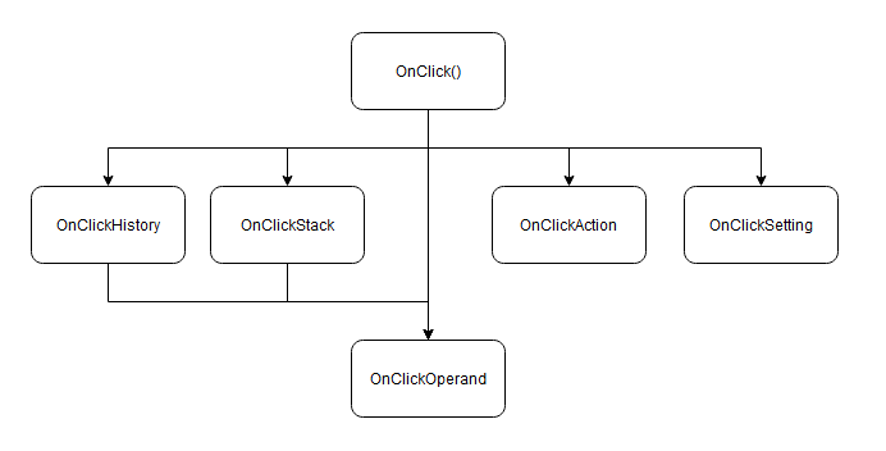
\includegraphics[width=1\columnwidth]{img/click-event-handling-vom-presenter}
	\caption[Click Event Handling vom Presenter]{Click Event Handling vom Presenter\footnotemark}
\end{figure}
\footnotetext{eigene Darstellung}

\interfootnotelinepenalty=100

\clearpage

\subsubsection{Planung der View [Tom]}

Für die Planung der View entschieden wir zuerst, dass die Applikation beim Start eine Kachelgestaltung in die Main Activity lädt. Dadurch erhält man eine Gridstruktur, in welcher die Kacheln unabhängig voneinander liegen. Diese Kachel geben ihren Inhalt an den Presenter weiter.

Dadurch, dass die Layouts angepasst werden können, muss das Laden dynamisch implementiert werden. Die Kacheln werden durch das Layout als Buttons mit Text generiert und setzt dann die Listeners aus dem Observer Pattern. Es gibt einen Kachelcontainer, welcher eine Liste aller Kacheln hat und eine Liste beider benötigten Stacks. Der Kachelcontainer soll mit Hilfe des Factory Patterns erstellt werden. Dabei wird ein String aus dem Speicher geladen und in den Container umgewandelt. Die Factory kann auch aus einem Layout den dazu passenden String erstellen und mit einer Bezeichnung versehen. 

Da die Kachel vom Kontext abhängig sind können diese nicht im Voraus geladen werden und es können keine Layouts gleichzeitig geladen werden. 

Es gibt ein Schema für Kacheln, damit diese nicht vom Kontext abhängig sind. Die Factory erstellt aus den Schemata konkrete Kacheln mit Typ und Inhalt. Der Inhalt muss an den Typ angepasst werden und damit die Kacheln nicht überladen werden können, werden Untertypen erstellt, die mit Hilfe eines Mappings ausgewählt werden können. Es werden erst beim Laden eines Layout die Schemata in tatsächliche Kacheln übertragen. Änderungen der Kacheln laufen auch exklusiv über die Schemata.

XXX ganz viele punkte

\clearpage

\subsubsection{Planung der Menüsteuerung [Istogu]}

Nachdem beschrieben wurde, wie die Planung für die Umsetzung der Anforderung erfolgte (''alle Kacheln sind gleichbedeutend, das heißt keine Kachel besitzt einen unveränderlichen Sonderstatus''\footnote{\cite[vgl.][]{seifert2020a}}) beschäftigt sich das folgende Unterkapitel mit der Anforderung, dass jeder Kachel jede Rolle zugewiesen werden kann.

In der Planungsphase wurde sich stärker an den Anforderung orientiert, zumal sie mögliche Implementierung skizzieren. Laut der Anforderung existiert ein Kacheltyp \code{CalculatorFunction}, der unter anderem ''auch die Zuordnung einer Funktionalität zu einer Kachel'' beinhaltet. Daher war die Idee, dass die Applikation zwei Activities beinhalten soll. Einmal eine Activity, die die Nutzung des Taschenrechners ermöglicht, und eine andere Activity, die einen ''Bearbeiten-Modus'' darstellen soll. Von dort aus könnte der Anwender sein Layout anpassen. Jedoch wurde diese Idee verworfen, weil sie auch mit den Anforderung teilweise kollidiert, dass die Funktionalitäten über eine minimale Menge von Interaktion erreicht werden soll. Stattdessen wurde entschieden den Ansatz zu verfolgen, der in der XXX Abbildung 7 zu sehen ist. Dieses Menü soll aufgerufen werden, wenn der Anwender eine Kachel länger gedrückt hält. 
Dabei soll ein Menü geöffnet werden, dass eine Auswahl an unterstützte Kacheltypen anbietet. Abhängig davon was ausgewählt wird, erscheint ein weiteres Untermenü. In der nachfolgende Abbildung wird dies anhand der Zuweisung eines Bruches verdeutlich. Die letzten Untermenüs dabei sind den Operanden vorbehalten.
 
\interfootnotelinepenalty=10000

\begin{figure}[!h]
	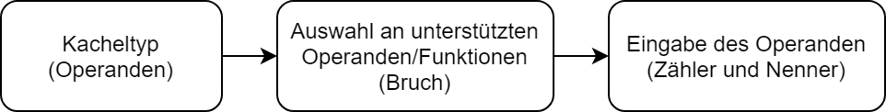
\includegraphics[width=1\columnwidth]{img/ablaufdiagramm-fuer-zuweisung}
	\caption[Ablaufdiagramm für die Zuweisung eines Bruches an einer Kachel]{Ablaufdiagramm für die Zuweisung eines Bruches an einer Kachel\footnotemark}
\end{figure}
\footnotetext{eigene Darstellung}

\interfootnotelinepenalty=100

XXX

%Nur eine Activity, die dynamisch aufgebaut und aktualisiert wird
%Dialoge, die zur Menüführung drübergelegt werden
%Argumente: Performance, Übersichtlichkeit, Lernzeit…

\clearpage

\subsection{Geplante Aufgabenverteilung im Team }

{\def\arraystretch{1.25}\tabcolsep=5pt
\begin{longtable}{|l|p{26em}|}
	\hline
	\textbf{Name} & \textbf{Aufgaben}
	\\ \hline \hline
	\endfirsthead
	
	\hline
	\endhead
	
	\hline
	\endfoot

	\textbf{Tim Schwenke} 
		& Einrichtung, Verwaltung und Bereitstellung der Versionsverwaltung \\
		& Architekturentwurf der Kalkulationsorchestrierung \\
		& LaTeX-Beauftragter \\
		& Projekttagebuch führen \\
		& Dokumentation anfertigen \\
	\hline
	\textbf{Hendrik Falk}
		& Gruppenweite Koordination des Projektes \\
		& Erstellung der simpelen Berechnungen und Sondertasten \\
		& Architekturentwurf der Front-End- und Back-End-Kommunikation \\
		& Projekttagebuch führen \\
		& Dokumentation anfertigen \\
	\hline
 	\textbf{Tim Meinerzhagen}
		& Planung und Implementierung der Java-Schnittstelle \\
		& Auswahl der zu verwendenden Math Bibliothek \\
		& Projekttagebuch führen \\
		& Dokumentation anfertigen \\
	\hline
	\textbf{Getuart Istogu}
		& Spezifikation und Dokumentation des Datenmodells und der Datenschnittstellen \\
		& Projekttagebuch führen \\
		& Dokumentation anfertigen \\
	\hline
	\textbf{Dennis Gentges}
		& Planung der Navigation zwischen den Activities und die einen Activity-Wechsel auslösenden Ereignisse \\
		& Projektplanung \\
		& Konzeptionierung der Benutzeroberfläche \\
		& Paper Prototype \\
		& Projekttagebuch führen \\
		& Dokumentation anfertigen \\
	\hline
	\textbf{Tom Bockhorn}
		& Planung der Navigation zwischen den Activities und die einen Activity-Wechsel auslösenden Ereignisse \\
		& Konzeptionierung der Benutzeroberfläche \\
		& Projekttagebuch führen \\
		& Dokumentation anfertigen \\
	\hline
	\textbf{Khang Pham}
		& Verantwortlichkeit für Erscheinungsbild der Arbeit, Vollständigkeit gemäß Gliederungsstruktur, Formatierung des Quellcodes im Anhang. \\
		& Konzeptionierung der Benutzeroberfläche \\
		& Projekttagebuch führen \\
		& Dokumentation anfertigen \\
	\hline
	\textbf{Jannis Luca Keienburg}
		& LaTeX-Beauftragter \\
		& Projekttagebuch führen \\
		& Dokumentation anfertigen \\
\end{longtable}
}